\documentclass[10pt]{beamer}\usepackage[]{graphicx}\usepackage[]{color}
% maxwidth is the original width if it is less than linewidth
% otherwise use linewidth (to make sure the graphics do not exceed the margin)
\makeatletter
\def\maxwidth{ %
  \ifdim\Gin@nat@width>\linewidth
    \linewidth
  \else
    \Gin@nat@width
  \fi
}
\makeatother

\definecolor{fgcolor}{rgb}{0.345, 0.345, 0.345}
\newcommand{\hlnum}[1]{\textcolor[rgb]{0.686,0.059,0.569}{#1}}%
\newcommand{\hlstr}[1]{\textcolor[rgb]{0.192,0.494,0.8}{#1}}%
\newcommand{\hlcom}[1]{\textcolor[rgb]{0.678,0.584,0.686}{\textit{#1}}}%
\newcommand{\hlopt}[1]{\textcolor[rgb]{0,0,0}{#1}}%
\newcommand{\hlstd}[1]{\textcolor[rgb]{0.345,0.345,0.345}{#1}}%
\newcommand{\hlkwa}[1]{\textcolor[rgb]{0.161,0.373,0.58}{\textbf{#1}}}%
\newcommand{\hlkwb}[1]{\textcolor[rgb]{0.69,0.353,0.396}{#1}}%
\newcommand{\hlkwc}[1]{\textcolor[rgb]{0.333,0.667,0.333}{#1}}%
\newcommand{\hlkwd}[1]{\textcolor[rgb]{0.737,0.353,0.396}{\textbf{#1}}}%
\let\hlipl\hlkwb

\usepackage{framed}
\makeatletter
\newenvironment{kframe}{%
 \def\at@end@of@kframe{}%
 \ifinner\ifhmode%
  \def\at@end@of@kframe{\end{minipage}}%
  \begin{minipage}{\columnwidth}%
 \fi\fi%
 \def\FrameCommand##1{\hskip\@totalleftmargin \hskip-\fboxsep
 \colorbox{shadecolor}{##1}\hskip-\fboxsep
     % There is no \\@totalrightmargin, so:
     \hskip-\linewidth \hskip-\@totalleftmargin \hskip\columnwidth}%
 \MakeFramed {\advance\hsize-\width
   \@totalleftmargin\z@ \linewidth\hsize
   \@setminipage}}%
 {\par\unskip\endMakeFramed%
 \at@end@of@kframe}
\makeatother

\definecolor{shadecolor}{rgb}{.97, .97, .97}
\definecolor{messagecolor}{rgb}{0, 0, 0}
\definecolor{warningcolor}{rgb}{1, 0, 1}
\definecolor{errorcolor}{rgb}{1, 0, 0}
\newenvironment{knitrout}{}{} % an empty environment to be redefined in TeX

\usepackage{alltt}


%\input{slides_header.tex}
\usepackage{graphicx}
\usepackage{hyperref, url}
\hypersetup{colorlinks,citecolor=myorange,filecolor=red,linkcolor=brown,urlcolor=blue}

\usepackage{longtable,booktabs}
\usepackage{amssymb,amsmath}
\usepackage{animate}
\usepackage{subfig}
\usepackage{tikz}
\usetikzlibrary{shapes.geometric, arrows,shapes.symbols,decorations.pathreplacing}
\tikzstyle{startstop} = [rectangle, rounded corners, minimum width=3cm, minimum height=1cm, draw=black, fill=pinkish,text width=3.5cm]
\tikzstyle{startstop2} = [rectangle, rounded corners, minimum width=3cm, minimum height=1cm, draw=black, fill=background,text width=4.5cm]
\tikzstyle{startstop3} = [rectangle, rounded corners, minimum width=3cm, minimum height=1cm, draw=black, fill=beige,text width=3.0cm]
\tikzstyle{startstop4} = [rectangle, rounded corners, minimum width=3cm, minimum height=1cm, draw=black, fill=pinkish,text width=4.5cm]
\tikzstyle{io} = [trapezium, trapezium left angle=70, trapezium right angle=110, minimum width=2cm, minimum height=1cm, text centered, draw=black, fill=blue!30,text width=1.5cm]
\tikzstyle{process} = [rectangle, minimum width=1cm, minimum height=1cm, text centered, draw=black, fill=orange!30,text width=2cm]
\tikzstyle{decision} = [diamond, minimum width=2cm, minimum height=1cm, text centered, draw=black, fill=green!30]
\tikzstyle{arrow} = [thick,->,>=stealth]
\tikzstyle{both} = [thick,<->,>=stealth, red]


% used for tree of stats tests in 001-introduction
\tikzstyle{startstopstats} = [rectangle, rounded corners, minimum width=2cm, minimum height=.5cm,text centered, draw=black, fill=red!30]
\tikzstyle{iostats} = [trapezium, trapezium left angle=70, trapezium right angle=110, minimum width=2cm, minimum height=.5cm, text centered, draw=black, fill=blue!30]
\tikzstyle{processstats} = [rectangle, minimum width=1.5cm, minimum height=.5cm, text centered, draw=black, fill=orange!30]
\tikzstyle{processbigstats} = [rectangle, minimum width=1.5cm, minimum height=.5cm, text centered, draw=black, fill=orange!30,text width=1.6cm]
\tikzstyle{decisionstats} = [rectangle, minimum width=1cm, minimum height=1cm, text centered, draw=black, fill=green!30,text width=1.6cm]
\tikzstyle{decisionbigstats} = [rectangle, minimum width=1cm, minimum height=1cm, text centered, draw=black, fill=yellow!30,text width=2cm]

\usepackage{pifont}% http://ctan.org/pkg/pifont
\newcommand{\cmark}{\ding{51}}%
\newcommand{\xmark}{\ding{55}}%

\usepackage{ulem} % for strikeout

\usepackage{xcolor}
\usepackage{color, colortbl}
\definecolor{lightgray}{RGB}{200,200,200}
\definecolor{palegray}{RGB}{221,221,221}
\definecolor{myblue}{RGB}{0,89,179}
\definecolor{myorange}{rgb}{0.776,0.357,0.157}
\definecolor{gray}{RGB}{110,110,110}
\definecolor{darkgray}{RGB}{100,100,100}
\definecolor{lightgray}{RGB}{200,200,200}
\definecolor{palegray}{RGB}{221,221,221}
\definecolor{turquoise}{RGB}{81,193,188}
\definecolor{tomato}{RGB}{255,136,136}
\definecolor{mandarina}{RGB}{229,169,25}
\definecolor{foreground}{RGB}{81,141,193}
\definecolor{background}{RGB}{246,244,240}
\definecolor{highlight}{RGB}{229,169,25}
\definecolor{lowlight}{RGB}{200,200,200}
\definecolor{beige}{RGB}{255,255,240}
\definecolor{pinkish}{RGB}{255,223,247}
\definecolor{darktangerine}{rgb}{1.0, 0.66, 0.07}
\definecolor{deepink}{RGB}{255,20,147}
%\usepackage{shadethm}
%\colorlet{shadecolor}{blue!15}
%\colorlet{shadecolor}{palegray}
%\setlength{\shadeboxrule}{.4pt}

%\newshadetheorem{thm}{Theorem}
%\newshadetheorem{defm}{Definition}
%\newshadetheorem{exm}{Exercise}
%\newshadetheorem{remarkm}{Remark}
%\definecolor{shadethmcolor}{HTML}{EDF8FF}
%\definecolor{shadethmcolor}{RGB}{221,221,221}
%\definecolor{shaderulecolor}{HTML}{45CFFF}
%\definecolor{shaderulecolor}{RGB}{0,89,179}
%\setlength{\shadeboxrule}{.4pt}



\usepackage{epsfig}

\newcommand{\code}[1]{\texttt{#1}}
\newcommand{\blue}[1]{\textcolor{blue}{#1}}
\newcommand{\red}[1]{\textcolor{red}{#1}}

\usepackage{comment}

\makeatletter

\def \iqsssectiontitleheader {}

\newcommand{\iqsssectiontitle}[1]{
	\def \iqsssectiontitleheader{#1}
}

\@ifundefined{insertmainframenumber}
{%
	% \insertmainframenumber not defined
	\newcommand{\insertmainframenumber}{\inserttotalframenumber}
}
{%
	% \insertmainframenumber already defined
}%


\AtBeginSection[]{
	\title{\insertsectionhead}
	{
		%\definecolor{white}{RGB}{140,193,250}
		%\definecolor{white}{RGB}{200,200,200}
		%\definecolor{white}{RGB}{242,244,247}
		\definecolor{white}{RGB}{0,89,179}
		%\definecolor{iqss@orange}{rgb}{1,1,1}
		\ifnum \insertmainframenumber > \insertframenumber
		%\setbeamercolor{background canvas}{bg=myblue}
		%\setbeamercolor{normal text}{fg=black,bg=white}
		%\setbeamercolor{frametitle}{fg=red}
		%\setbeamercolor{section in toc}{fg=myblue, bg=white}
		%\setbeamercolor{subsection in toc}{fg=myblue, bg=white}
		\frame{
			\frametitle{\iqsssectiontitleheader}
			\tableofcontents[currentsection]
		}
		\else
		\frame{
			\frametitle{Backup Slides}
			\tableofcontents[sectionstyle=shaded/shaded,subsectionstyle=shaded/shaded/shaded]
		}
		\fi
	}
}
\makeatother
%\graphicspath{{/home/sahir/git_repositories/EPIB607/resources/assets/slides/figure/}}


\usepackage{fontspec}
%\setsansfont{Fira Sans}
%\setmonofont{Fira Mono}
%\setsansfont[ItalicFont={Fira Sans Light Italic},BoldFont={Fira Sans},BoldItalicFont={Fira Sans Italic}]{Fira Sans Light}
%\setmonofont[BoldFont={Fira Mono Medium}]{Fira Mono}

\def\installpath{/usr/local/share/texmf/fonts/opentype/libertinus/}
\setmainfont{LibertinusSerif}[
UprightFont    = *-Regular,
BoldFont       = *-Bold,
ItalicFont     = *-Italic,
BoldItalicFont = *-BoldItalic,
Ligatures      = TeX,
Extension      = .otf,
Path           = \installpath/
]

\setsansfont{LibertinusSerif}[
UprightFont    = *-Regular,
BoldFont       = *-Bold,
ItalicFont     = *-Italic,
BoldItalicFont = *-BoldItalic,
Ligatures      = TeX,
Extension      = .otf,
Path           = \installpath/
]


%\setmonofont{LibertinusSerif}[
%UprightFont    = *-Regular,
%BoldFont       = *-Bold,
%ItalicFont     = *-Italic,
%BoldItalicFont = *-BoldItalic,
%Ligatures      = TeX,
%Extension      = .otf,
%Path           = \installpath/
%]






\newcommand\Wider[2][3em]{%
	\makebox[\linewidth][c]{%
		\begin{minipage}{\dimexpr\textwidth+#1\relax}
			\raggedright#2
		\end{minipage}%
	}%
}


\newcommand {\framedgraphic}[1] {
	\begin{figure}
		\centering
		\includegraphics[width=\textwidth,height=0.9\textheight,keepaspectratio]{#1}
	\end{figure}
}


\newcommand {\framedgraphiccaption}[2] {
	\begin{figure}
		\centering
		\includegraphics[width=\textwidth,height=0.8\textheight,keepaspectratio]{#1}
		\caption{#2}
	\end{figure}
}




\setbeamercolor{itemize item}{fg=myblue}
\setbeamercolor{itemize subitem}{fg=myorange}
%\setbeamertemplate{itemize item}[square]
\setbeamertemplate{itemize item}[circle]
\setbeamertemplate{itemize subitem}[triangle]
\setbeamertemplate{blocks}[rounded][shadow=true]
\setbeamercolor{block body alerted}{bg=alerted text.fg!10}
\setbeamercolor{block title alerted}{bg=alerted text.fg!20}
\setbeamercolor{block body}{bg=structure!10}
\setbeamercolor{block title}{bg=structure!20}
\setbeamercolor{block body example}{bg=green!10}
\setbeamercolor{block title example}{bg=green!20}


\makeatletter
\newenvironment<>{proofs}[1][\proofname]{%
	\par
	\def\insertproofname{#1\@addpunct{.}}%
	\usebeamertemplate{proof begin}#2}
{\usebeamertemplate{proof end}}
\newenvironment<>{proofc}{%
	\setbeamertemplate{proof begin}{\begin{block}{}}
		\par
		\usebeamertemplate{proof begin}}
	{\usebeamertemplate{proof end}}
	\newenvironment<>{proofe}{%
		\par
		\pushQED{\qed}
		\setbeamertemplate{proof begin}{\begin{block}{}}
			\usebeamertemplate{proof begin}}
		{\popQED\usebeamertemplate{proof end}}
\makeatother


\makeatletter
\newenvironment<>{exams}[1][\proofname]{%
	\par
	\def\insertproofname{#1\@addpunct{.}}%
	\usebeamertemplate{example begin}#2}
{\usebeamertemplate{example end}}
\newenvironment<>{examc}{%
	\setbeamertemplate{exam begin}{\begin{block}{}}
		\par
		\usebeamertemplate{exam begin}}
	{\usebeamertemplate{exam end}}
	\newenvironment<>{exame}{%
		\par
		\pushQED{\qed}
		\setbeamertemplate{exam begin}{\begin{block}{}}
			\usebeamertemplate{exam begin}}
		{\popQED\usebeamertemplate{exam end}}
		\makeatother

%\definecolor{mycolor}{HTML}{F7F8E0}
%\declaretheorem[shaded={bgcolor=mandarina}]{theo}
%\declaretheorem[shaded={bgcolor=mycolor}]{propo}
%\declaretheorem[shaded={bgcolor=green!80!black!30}]{remark}

%\setbeamertemplate{navigation symbols}{\usebeamercolor[fg]{title in head/foot}\usebeamerfont{title in head/foot}\insertframenumber}


%\setbeamertemplate{footline}{}

\beamertemplatenavigationsymbolsempty % toggle off if you want navigation symbols at the bottom

\setbeamertemplate{footline}
{ \usebeamercolor[fg]{page number in head/foot}%
	\usebeamerfont{page number in head/foot}%
	\hspace{1em}\insertsectionhead%
	\hfill%
	\insertframenumber\,/\,\hyperlinkappendixstart{\insertmainframenumber}
	\ifnum \thepage = \insertframeendpage{\small .}\else{\phantom{\small .}}\fi
	\hspace{1em}
	\vskip2pt%
}

%\newtheorem{proposition}[theorem]{Proposition}
%\newtheorem{exercise}[theorem]{Exercise}
%\newtheorem{remark}[theorem]{Remark}


\usepackage{amsthm}
\usepackage{thmtools}

\setbeamertemplate{theorems}[ams style] 
%\setbeamertemplate{theorems}[numbered] 
%\setbeamertemplate{corollary}[numbered] 
\newtheorem{proposition}{Proposition}
\newtheorem{exercise}{Exercise}
\newtheorem{remark}{Remark}
\newtheorem{exam}{Example}
%\newtheorem{proof}{Proof}
%\newtheorem{corollaries}[theorem]{Corollary}
\newcommand*{\theorembreak}{\usebeamertemplate{theorem end}\framebreak\usebeamertemplate{theorem begin}}



\setlength{\emergencystretch}{3em} % prevent overfull lines
\providecommand{\tightlist}{%
	\setlength{\itemsep}{0pt}\setlength{\parskip}{0pt}}

\newcommand\AddButton{%
	\setbeamertemplate{background canvas}{%
		\begin{tikzpicture}[remember picture,overlay]
		\node[anchor=west] at ([yshift=5pt,xshift=0.1em]current page.south west)
		{\hyperlink{toc}{\beamergotobutton{back to TOC}}};
		\end{tikzpicture}%
	}%
}


\titlegraphic{\hfill
\includegraphics[height=1cm]{/home/sahir/git_repositories/EPIB607/slides/mcgill_logo.png}}




\graphicspath{{/home/sahir/git_repositories/EPIB607/slides/figure/}}
%\newtheorem*{remark}{Remark}

%\let\oldShaded\Shaded
%\let\endoldShaded\endShaded
%\renewenvironment{Shaded}{\footnotesize\oldShaded}{\endoldShaded}

\newcommand{\Var}{\operatorname{Var}}
\newcommand{\Expec}{\operatorname{E}}
\newcommand{\Prob}{\operatorname{P}}
\IfFileExists{upquote.sty}{\usepackage{upquote}}{}
\begin{document}
	
	
	
	%\title{Introduction to Regression Trees}
	%\author{Sahir Bhatnagar \inst{1}}
	%\author[shortname]{Sahir Rai Bhatnagar, PhD Candidate (Biostatistics) }
	%\institute[shortinst]{Department of Epidemiology, Biostatistics and Occupational Health}
	
	\title{014 - Bootstrap Confidence Intervals}
	\author{EPIB 607}
	\institute{
		Sahir Rai Bhatnagar\\
		Department of Epidemiology, Biostatistics, and Occupational Health\\
		McGill University\\
		
		\vspace{0.1 in}
		
		\texttt{sahir.bhatnagar@mcgill.ca}\\
		%\texttt{\url{https://sahirbhatnagar.com/EPIB607/}}
	}
	
	\date{slides compiled on \today}
	
	\maketitle

%\section{Objectives}

\section{Review of Confidence Intervals}

\begin{frame}{Sampling Distribution}
	
	\begin{definition}[Sampling Distribution]
		\begin{itemize}
			\item The sampling distribution of a statistic is the distribution of values taken by the statistic in \textbf{all possible samples of the same size} from the same population.
			\item The standard deviation of a sampling distribution is called a \textbf{standard error}
		\end{itemize} 
	\end{definition}
	
	
\end{frame}


\begin{frame}[fragile]{Sampling Distributions}
	
\begin{knitrout}\tiny
\definecolor{shadecolor}{rgb}{0.969, 0.969, 0.969}\color{fgcolor}\begin{figure}

{\centering 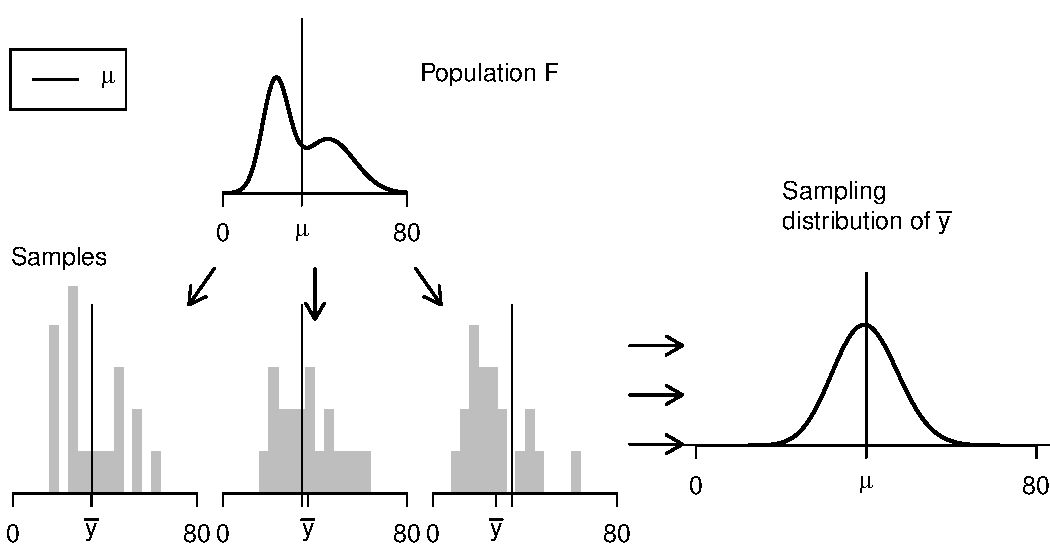
\includegraphics[width=\maxwidth]{figure/unnamed-chunk-1-1} 

}

\caption[Ideal world]{Ideal world. Sampling distributions are obtained by drawing repeated samples from the population, computing the statistic of interest for each, and collecting (an infinite number of) those statistics as the sampling distribution}\label{fig:unnamed-chunk-1}
\end{figure}

\end{knitrout}
	
\end{frame}



\begin{frame}{Sampling Distribution}
	
	\Wider[4em]{
		\begin{figure}
			\centering
			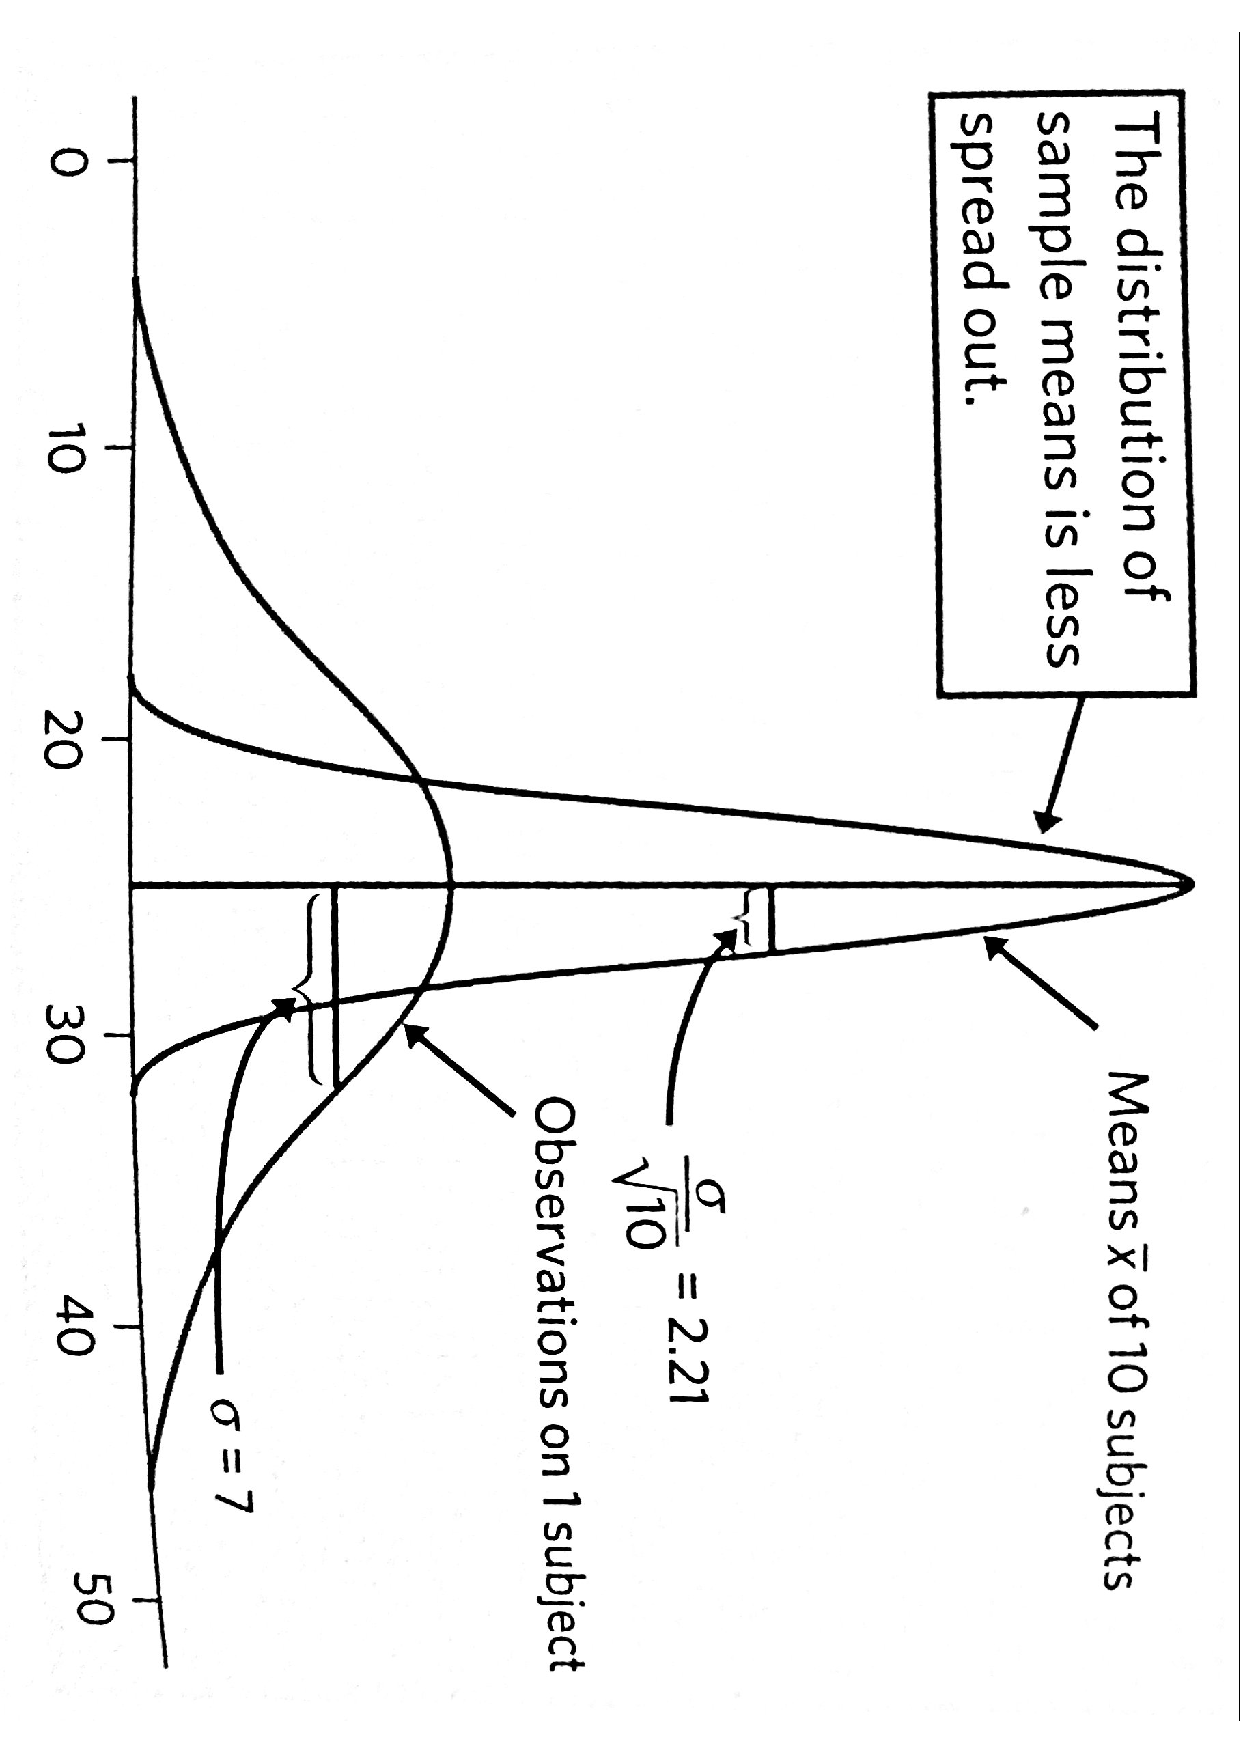
\includegraphics[scale=0.33, angle=90]{samplingdist_B_M.pdf}
			\caption{Averages are less variable than individual observations}
		\end{figure}
	}
	
\end{frame}



\frame{\frametitle{Traditional way to calculate CIs}
	How to construct a CI for the population mean?
	\begin{itemize}
		\item The \textbf{CLT} gives us that $\overline{y} \sim
		\mathcal{N}(\mu,\sigma/\sqrt{n})$ is approximately true when $n$ is
		large. 
		\item We can standardize, to get $Z = \frac{\overline{y}-\mu}{\sigma/\sqrt{n}} \sim
		\mathcal{N}(0,1)$. 
		\item To find a CI with confidence level $\mathcal{C} = 1-\alpha$, we must calculate the critical value $z^*$  such that \begin{equation}
		P(-z^* < Z < z^*) = \mathcal{C} = 1-\alpha
		\end{equation}
		where $\alpha$ is the significance level 
		\begin{itemize}
			\item That is, we want the value $z^*$ that gives a
			\textit{lower tail probability} of $(1-\mathcal{C})/2 = \alpha / 2$. 
			\item Often this value is denoted $z^* = z_{\alpha/2}$; thus we have \[P(Z <
			-z_{\alpha/2}) = \alpha/2,\] and \[P(Z >
			z_{\alpha/2}) = \alpha/2.\]
		\end{itemize}
	\end{itemize}
} 

\begin{comment}
\frame{\frametitle{CIs for $\mu$ when $\sigma^2$ is known} Then we
have:
\[\begin{array}{ccl} 1-\alpha & = & P(-z_{\alpha/2} < Z < z_{\alpha/2})\\
& & \\ & = & P\left(-z_{\alpha/2} < \frac{\overline{y}-\mu}{\sigma/\sqrt{n}} < z_{\alpha/2}\right)\\
& & \\ & = & P\left(-z_{\alpha/2} <
\frac{\mu-\overline{y}}{\sigma/\sqrt{n}} <
z_{\alpha/2}\right)\\ \pause
& & \\ & = & P\left(-z_{\alpha/2}\frac{\sigma}{\sqrt{n}} <
\mu-\overline{y} <
z_{\alpha/2}\frac{\sigma}{\sqrt{n}}\right)\\ \pause
& & \\ & = & P\left(\overline{y}-z_{\alpha/2}\frac{\sigma}{\sqrt{n}}
< \mu < \overline{y}+z_{\alpha/2}\frac{\sigma}{\sqrt{n}}\right)\\ & & \\
\end{array}\]

So a $(1-\alpha)$100\% CI for $\mu$ is
\textcolor{blue}{$\overline{y}\pm
z_{\alpha/2}\frac{\sigma}{\sqrt{n}}$.} }
\end{comment}

\begin{frame}{Traditional way to calculate CIs}
	
	\Wider[2em]{
		
		
		\begin{columns}
			\begin{column}{0.5\textwidth}
				\begin{figure}
					\centering
					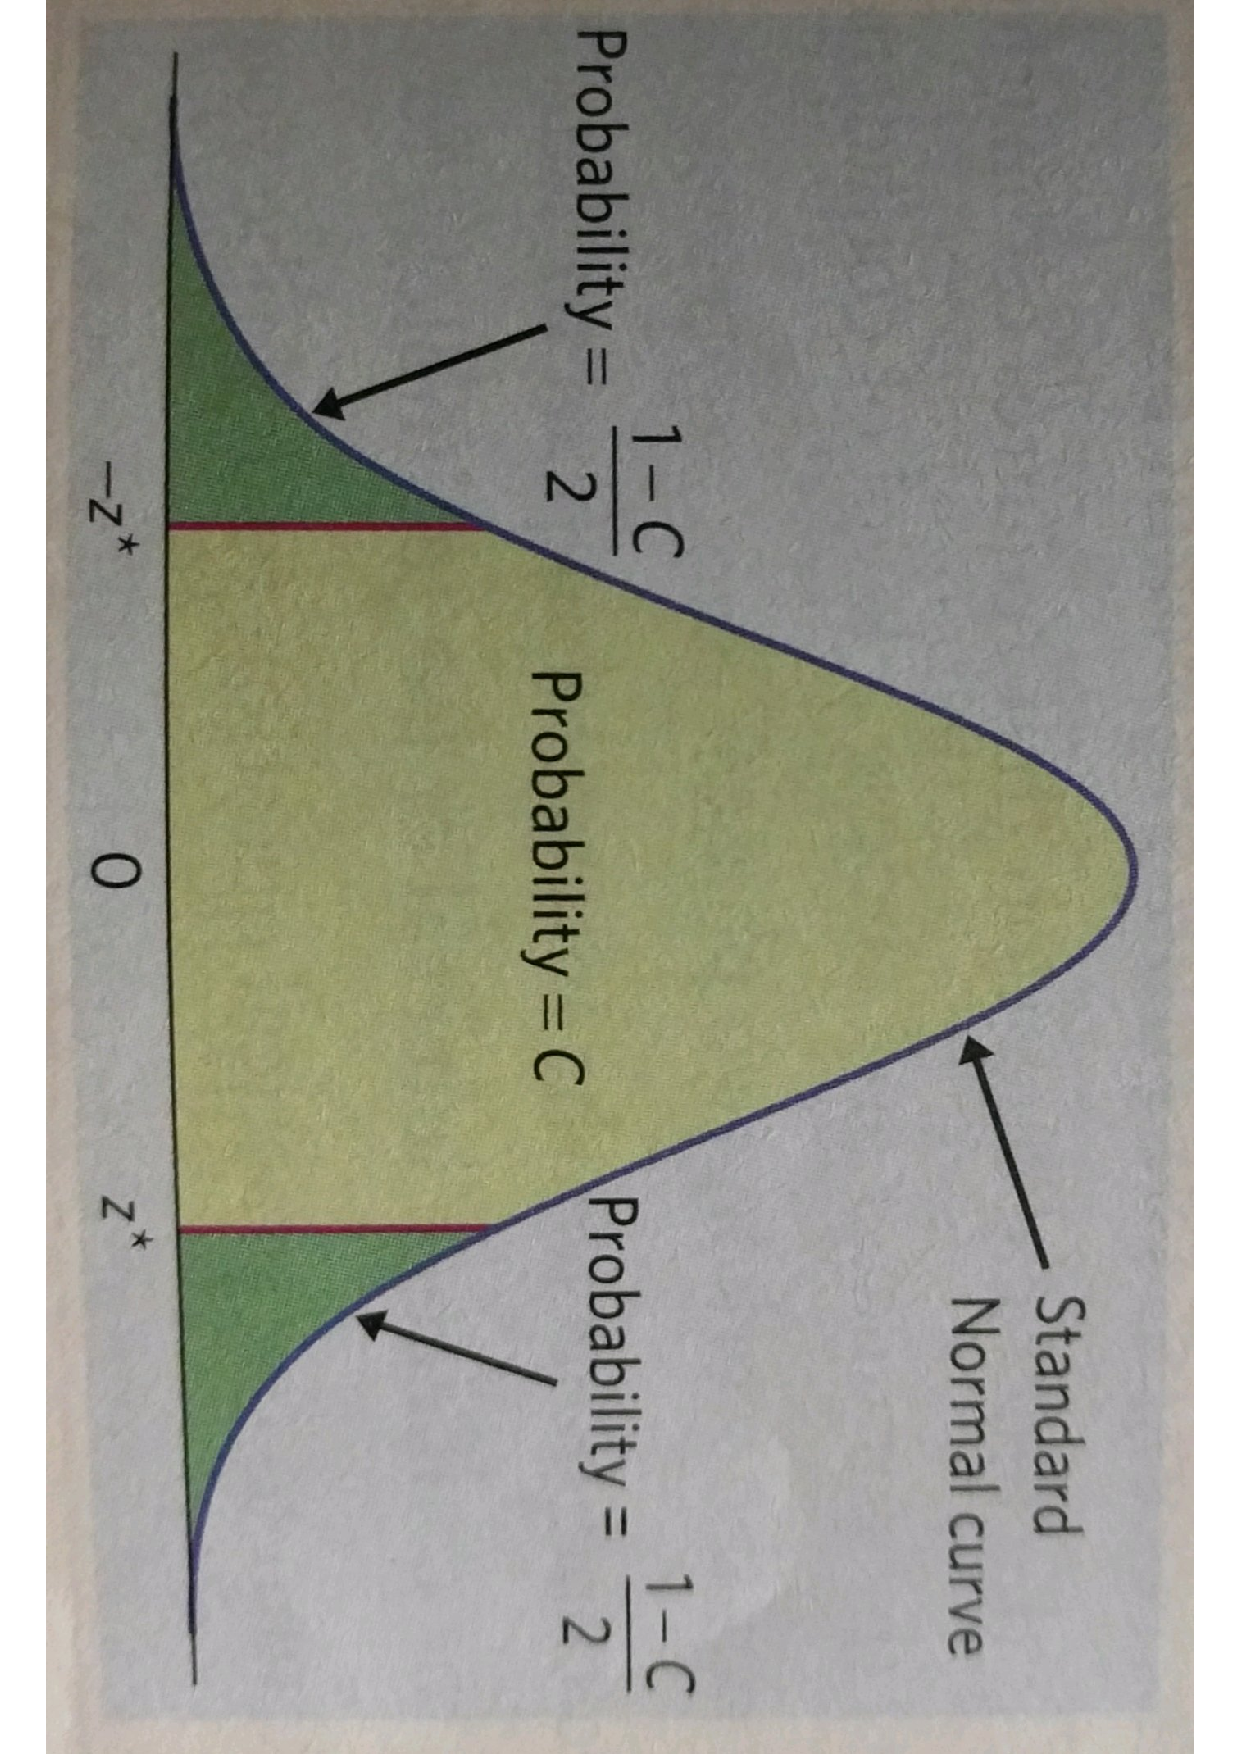
\includegraphics[scale=0.15, angle=90]{normal.pdf}
					\caption{\small The critical value $z^\star$ is the number that catches central probability $\mathcal{C}$ under a standard normal $\mathcal{N}(0,1)$ curve between $-z^\star$ and $z^\star$}
				\end{figure}
			\end{column}
			\begin{column}{0.5\textwidth}  %%<--- here
				\scriptsize
				We can use this probability statement about the \underline{standardized version} of the sample mean
				$(\bar{y} - \mu )/ \sigma / \sqrt{n}$, to place bounds on where we think the true mean lies
				by examining the probability that $\bar{y}$ is within
				$z^\star \cdot \frac{\sigma}{\sqrt{n}}$ of $\mu$ \\ 
				\begin{align*}
				\mathcal{C} & = P\left(-z^\star \le \frac{\bar{y}-\mu}{\sigma/\sqrt{n}} \le
				z^\star\right)\\
				& = P\left(-z^\star\frac{\sigma}{\sqrt{n}}
				\le \bar{y}-\mu \le +z^\star\frac{\sigma}{\sqrt{n}}\right)\\	
				& = P\left(-\bar{y}-z^\star\frac{\sigma}{\sqrt{n}} \le
				-\mu \le -\bar{y}+z^\star\frac{\sigma}{\sqrt{n}}\right)\\ 
				& = P\left(\bar{y}+z^\star\frac{\sigma}{\sqrt{n}} \ge
				\mu \ge \bar{y}-z^\star\frac{\sigma}{\sqrt{n}}\right)\\ 
				& = P\left(\bar{y}-z^\star\frac{\sigma}{\sqrt{n}} \le \mu
				\le \bar{y}+z^\star\frac{\sigma}{\sqrt{n}}\right)\\
				& = 1-\alpha
				\end{align*}
				
				We call the interval
				$\left(\bar{y}-z^\star\frac{\sigma}{\sqrt{n}},
				\bar{y}+z^\star\frac{\sigma}{\sqrt{n}}\right)$ a \textbf{(1-$\alpha$)100\%
					confidence interval} for $\mu$.
			\end{column}
		\end{columns}
		
		
	}
	
\end{frame}







\begin{frame}[fragile]{Confidence intervals for depths of the ocean}
	
	\vspace*{-0.19in}
	
	
\begin{knitrout}\tiny
\definecolor{shadecolor}{rgb}{0.969, 0.969, 0.969}\color{fgcolor}\begin{figure}

{\centering 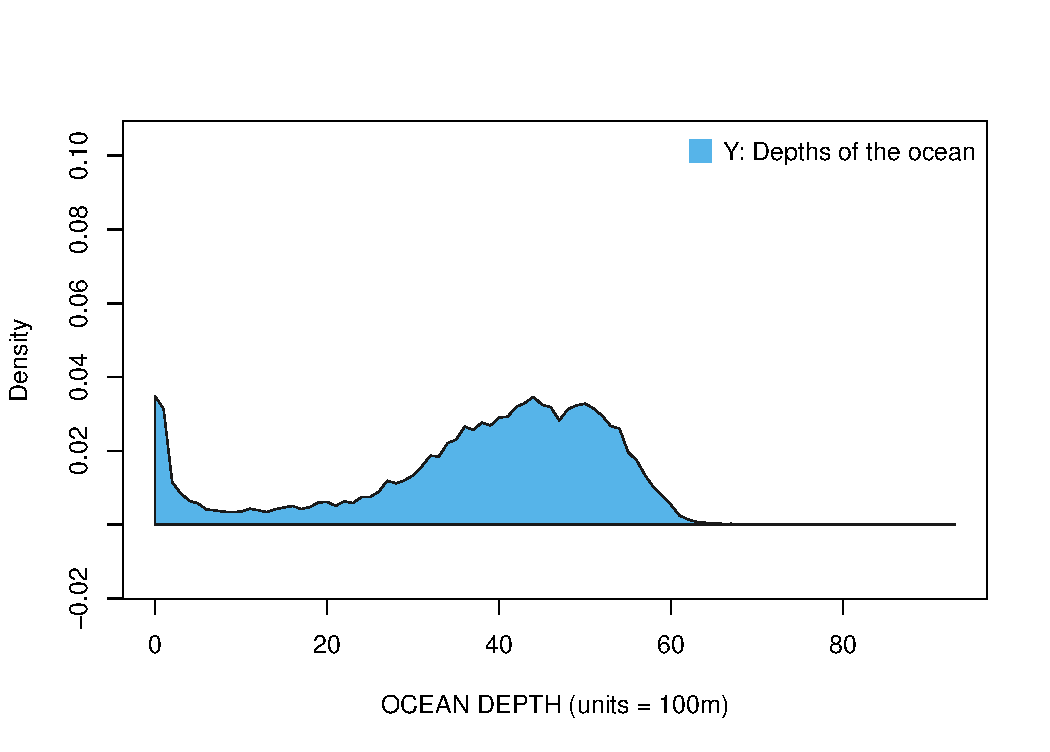
\includegraphics[width=\maxwidth]{figure/unnamed-chunk-2-1} 

}

\caption[The original data distribution of sampled depths of the ocean]{The original data distribution of sampled depths of the ocean. Note that it has multiple modes and not Normal looking.}\label{fig:unnamed-chunk-2}
\end{figure}

\end{knitrout}
	
	
\end{frame}



\begin{frame}[fragile]{The CLT is 'kicking in' at $n=16$}
	
	\vspace*{-0.09in}
	
	
\begin{knitrout}\tiny
\definecolor{shadecolor}{rgb}{0.969, 0.969, 0.969}\color{fgcolor}\begin{figure}

{\centering 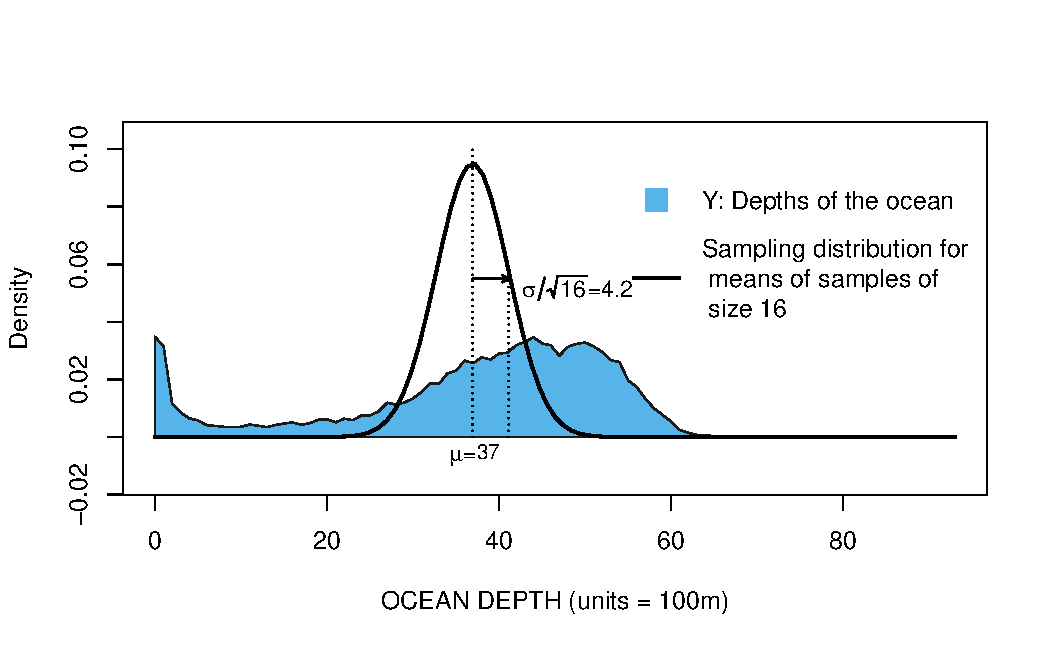
\includegraphics[width=\maxwidth]{figure/unnamed-chunk-3-1} 

}

\caption[The sampling distribution for the mean depth of the ocean with samples of size $n=16$, looks normal (centered at $\mu=37$ and SD equal to $\sigma/\sqrt{16}$) ]{The sampling distribution for the mean depth of the ocean with samples of size $n=16$, looks normal (centered at $\mu=37$ and SD equal to $\sigma/\sqrt{16}$) }\label{fig:unnamed-chunk-3}
\end{figure}

\end{knitrout}
	
\end{frame}


\begin{frame}[fragile]{Since CLT has 'kicked in', we use it to construct a CI}
	\small
	We want to construct a $\mathcal{C} = 95\%$ confidence interval for the mean. Level of significance is $\alpha = 1-\mathcal{C} = 0.05$ \pause
	
	\begin{enumerate}
		\setlength\itemsep{1em}
		\item by the CLT $\to$ $\bar{y} \sim \mathcal{N}(mean = 37, sd = \sigma/\sqrt{16} = 4.2)$ \pause
		\item The critical value $z^\star$ such that $P(Z < -z^\star) = P(Z > z^\star) = \alpha/2 = 0.025$ is given by 
\begin{knitrout}\tiny
\definecolor{shadecolor}{rgb}{0.969, 0.969, 0.969}\color{fgcolor}\begin{kframe}
\begin{alltt}
\hlstd{mosaic}\hlopt{::}\hlkwd{xqnorm}\hlstd{(}\hlkwc{p} \hlstd{=} \hlkwd{c}\hlstd{(}\hlnum{0.025}\hlstd{,} \hlnum{0.975}\hlstd{))}
\end{alltt}
\end{kframe}

{\centering 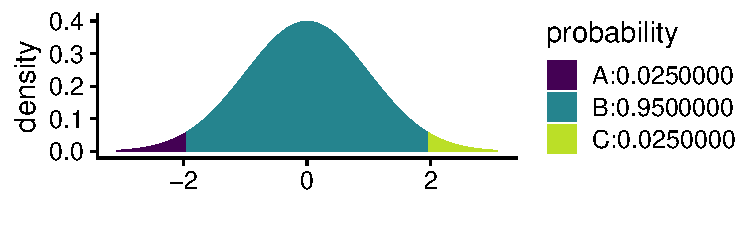
\includegraphics[width=\maxwidth]{figure/unnamed-chunk-4-1} 

}


\begin{kframe}\begin{verbatim}
## [1] -1.959964  1.959964
\end{verbatim}
\end{kframe}
\end{knitrout}
		\pause
		\item 95\% CI for $\mu$: $(37 - 1.96 \cdot 4.2, 37 + 1.96 \cdot 4.2) = [29, 45]$
	\end{enumerate}
\end{frame}


\begin{frame}{Alternative way of calculating CI with CLT: \texttt{qnorm}}
	
	\begin{itemize}
		\setlength\itemsep{1em}
		\item In the previous slides we used the standard normal $\mathcal{N}(0, 1)$ to calculate the critical value $z^\star$ needed for the CI
		\item We were able to use the $\mathcal{N}(0,1)$ for two reasons: \pause
		\begin{enumerate}
			\item the CLT \pause 
			\item the formula used to calculate the CI is based on standardizing $\bar{y} \to \frac{\bar{y} - \mu}{\sigma / \sqrt{n}}$
		\end{enumerate}
	\end{itemize}
	\pause 
	
	\begin{itemize}
		\setlength\itemsep{1em}
		\item There is an alternative, \textbf{yet equivalent}, way to calculate the CI without standardizing $\bar{y}$, and without using the $\pm$ formula \pause
		\item This is accomplished using \texttt{qnorm} \pause 
		\item Note: we \textbf{still need the CLT regardless} of whether we use the $\pm$ formula or \texttt{qnorm}
	\end{itemize}
	
\end{frame}


\begin{frame}[fragile]{68\% Confidence interval using \texttt{qnorm}}
	
	\vspace*{-0.09in}
	
	\Wider[2em]{
\begin{knitrout}\tiny
\definecolor{shadecolor}{rgb}{0.969, 0.969, 0.969}\color{fgcolor}\begin{figure}

{\centering 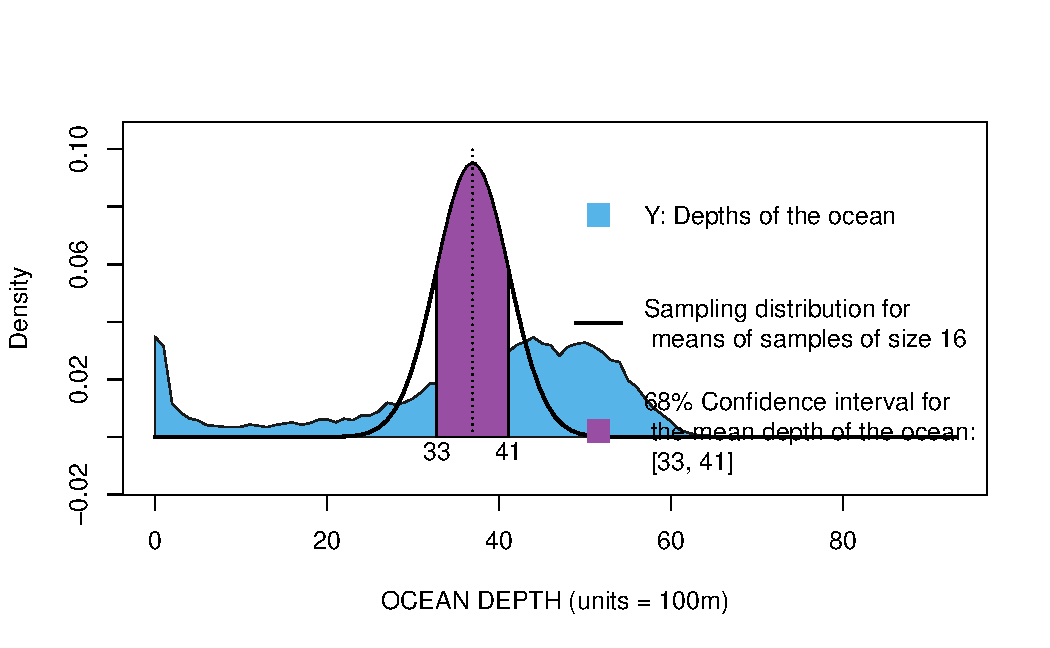
\includegraphics[width=\maxwidth]{figure/unnamed-chunk-5-1} 

}

\caption{68\% Confidence interval calculated using  \mbox{\texttt{qnorm(p = c(0.16,0.84), mean = 37, sd = 4.2)}}}\label{fig:unnamed-chunk-5}
\end{figure}

\end{knitrout}
		
	}
\end{frame}



\begin{frame}[fragile]{95\% Confidence interval using \texttt{qnorm}}
	
	\vspace*{-0.09in}
	
	
	\Wider[2em]{
\begin{knitrout}\tiny
\definecolor{shadecolor}{rgb}{0.969, 0.969, 0.969}\color{fgcolor}\begin{figure}

{\centering 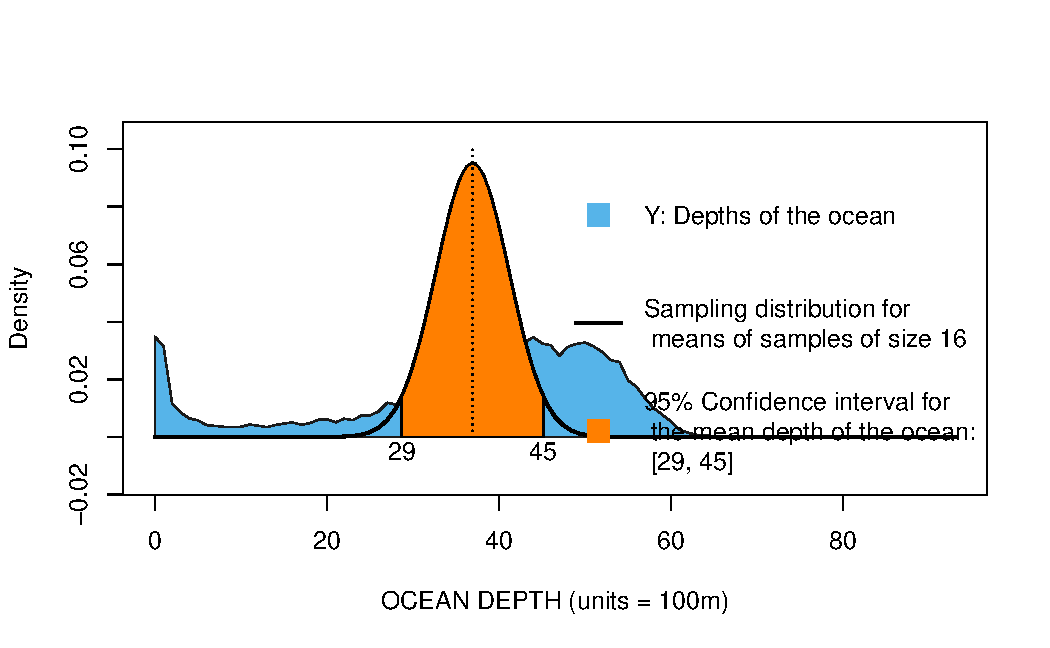
\includegraphics[width=\maxwidth]{figure/unnamed-chunk-6-1} 

}

\caption{95\% Confidence interval calculated using  \mbox{\texttt{qnorm(p = c(0.025,0.975), mean = 37, sd = 4.2)}}}\label{fig:unnamed-chunk-6}
\end{figure}

\end{knitrout}
		
	}
	
\end{frame}


\begin{frame}{Motivation for the Bootstrap}
	\begin{itemize}
		\setlength\itemsep{2em}
		\item The $\pm$ and \texttt{qnorm} methods to calculate a CI both require the CLT
	\end{itemize}
	
	\pause
	
	\vspace*{0.2in}
	
	\Large \textcolor{myblue}{Q: What happens if the CLT hasn't `kicked in`? Or you don't believe the CLT?} \\ \ \\
	\pause 
	\Large \textcolor{red}{A: Bootstrap} \\ \ \\
\end{frame}


\section{The Bootstrap}


\begin{frame}[fragile]{Ideal world: known sampling distribution}
	
\begin{knitrout}\tiny
\definecolor{shadecolor}{rgb}{0.969, 0.969, 0.969}\color{fgcolor}\begin{figure}

{\centering 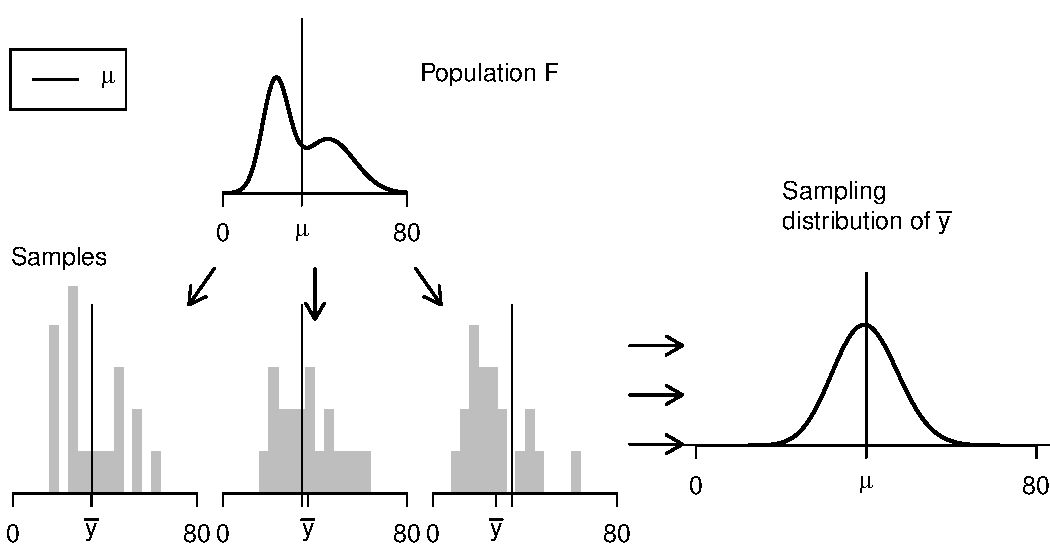
\includegraphics[width=\maxwidth]{figure/unnamed-chunk-7-1} 

}

\caption{\scriptsize{Ideal world. Sampling distributions are obtained by drawing repeated samples from the population, computing the statistic of interest for each, and collecting (an infinite number of) those statistics as the sampling distribution}}\label{fig:unnamed-chunk-7}
\end{figure}

\end{knitrout}
	
\end{frame}



\begin{frame}[fragile]{Reality: use the bootstrap distribution instead}
	
	

	
	\framedgraphiccaption{boot_diag.pdf}{\scriptsize{Bootstrap world. The bootstrap distribution is obtained by drawing repeated samples from an estimate of the population, computing the statistic of interest for each, and collecting those statistics. The distribution is centered at the observed statistic ($\bar{y}$), not the parameter ($\mu$).}}
	
\end{frame}


\begin{frame}[fragile]{Main idea: simulate your own sampling distribution}
	

	
\begin{knitrout}\tiny
\definecolor{shadecolor}{rgb}{0.969, 0.969, 0.969}\color{fgcolor}\begin{kframe}
\begin{alltt}
\hlstd{R} \hlkwb{<-} \hlkwd{replicate}\hlstd{(B, \{}
  \hlstd{dplyr}\hlopt{::}\hlkwd{sample_n}\hlstd{(depths.n.20,} \hlkwc{size} \hlstd{= N,} \hlkwc{replace} \hlstd{=} \hlnum{TRUE}\hlstd{)} \hlopt
  \hlstd{dplyr}\hlopt{::}\hlkwd{summarize}\hlstd{(}\hlkwc{r} \hlstd{=} \hlkwd{mean}\hlstd{(alt))} \hlopt
  \hlstd{dplyr}\hlopt{::}\hlkwd{pull}\hlstd{(r)}
\hlstd{\})}
\hlstd{CI_95} \hlkwb{<-} \hlkwd{quantile}\hlstd{(R,} \hlkwc{probs} \hlstd{=} \hlkwd{c}\hlstd{(}\hlnum{0.025}\hlstd{,} \hlnum{0.975}\hlstd{))}
\end{alltt}
\end{kframe}

{\centering 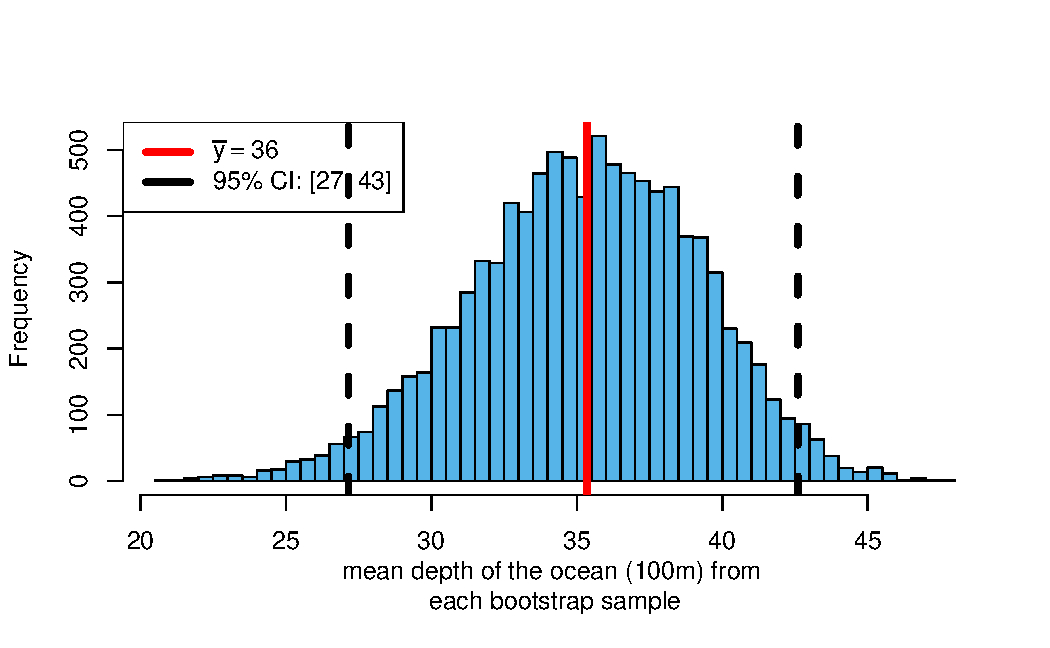
\includegraphics[width=\maxwidth]{figure/unnamed-chunk-10-1} 

}


\end{knitrout}
	
\end{frame}


\begin{frame}[fragile]{Bootstrap code 1}
	
\begin{knitrout}\tiny
\definecolor{shadecolor}{rgb}{0.969, 0.969, 0.969}\color{fgcolor}\begin{kframe}
\begin{alltt}
\hlcom{# function for sampling ocean depths}
\hlkwd{source}\hlstd{(}\hlstr{"https://raw.githubusercontent.com/sahirbhatnagar/EPIB607/master/labs/
      003-ocean-depths/automate_water_task.R"}\hlstd{)}

\hlcom{# from the in-class exercise}
\hlstd{index.n.20} \hlkwb{<-} \hlkwd{c}\hlstd{(}\hlnum{2106}\hlstd{,}\hlnum{2107}\hlstd{,}\hlnum{2108}\hlstd{,}\hlnum{2109}\hlstd{,}\hlnum{2110}\hlstd{,}\hlnum{2111}\hlstd{,}\hlnum{2112}\hlstd{,}
\hlnum{2113}\hlstd{,}\hlnum{2114}\hlstd{,}\hlnum{2115}\hlstd{,}\hlnum{2116}\hlstd{,}\hlnum{2117}\hlstd{,}\hlnum{2118}\hlstd{,}\hlnum{2119}\hlstd{,}
\hlnum{2120}\hlstd{,}\hlnum{2121}\hlstd{,}\hlnum{2122}\hlstd{,}\hlnum{2123}\hlstd{,}\hlnum{2124}\hlstd{,}\hlnum{2125}\hlstd{)}

\hlcom{# get depths of ocean sample n=20}
\hlstd{depths.n.20} \hlkwb{<-} \hlkwd{automate_water_task}\hlstd{(}\hlkwc{index} \hlstd{= index.n.20,}
               \hlkwc{student_id} \hlstd{=} \hlnum{260194225}\hlstd{,} \hlkwc{type} \hlstd{=} \hlstr{"depth"}\hlstd{)}

\hlcom{# change to 100m units}
\hlstd{depths.n.20}\hlopt{$}\hlstd{alt} \hlkwb{=} \hlkwd{round}\hlstd{(depths.n.20}\hlopt{$}\hlstd{alt}\hlopt{/}\hlnum{100}\hlstd{,}\hlnum{0}\hlstd{)}

\hlstd{B} \hlkwb{<-} \hlnum{10000}\hlstd{; N} \hlkwb{<-} \hlkwd{nrow}\hlstd{(depths.n.20)}
\hlstd{R} \hlkwb{<-} \hlkwd{replicate}\hlstd{(B, \{}
\hlstd{dplyr}\hlopt{::}\hlkwd{sample_n}\hlstd{(depths.n.20,} \hlkwc{size} \hlstd{= N,} \hlkwc{replace} \hlstd{=} \hlnum{TRUE}\hlstd{)} \hlopt
\hlstd{dplyr}\hlopt{::}\hlkwd{summarize}\hlstd{(}\hlkwc{r} \hlstd{=} \hlkwd{mean}\hlstd{(alt))} \hlopt
\hlstd{dplyr}\hlopt{::}\hlkwd{pull}\hlstd{(r)}
\hlstd{\})}

\hlstd{CI_95} \hlkwb{<-} \hlkwd{quantile}\hlstd{(R,} \hlkwc{probs} \hlstd{=} \hlkwd{c}\hlstd{(}\hlnum{0.025}\hlstd{,} \hlnum{0.975}\hlstd{))}
\end{alltt}
\end{kframe}
\end{knitrout}
	
	
\end{frame}

\begin{frame}[fragile]{Bootstrap code 2}
	
\begin{knitrout}\tiny
\definecolor{shadecolor}{rgb}{0.969, 0.969, 0.969}\color{fgcolor}\begin{kframe}
\begin{alltt}
\hlcom{# plot sampling distribution}
\hlkwd{hist}\hlstd{(R,} \hlkwc{breaks} \hlstd{=} \hlnum{50}\hlstd{,} \hlkwc{col} \hlstd{=} \hlstr{"#56B4E9"}\hlstd{,}
\hlkwc{main}\hlstd{=}\hlstr{""}\hlstd{,}
\hlkwc{xlab} \hlstd{=} \hlstr{"mean depth of the ocean (100m) from each bootstrap sample"}\hlstd{)}

\hlcom{# draw red line at the sample mean}
\hlkwd{abline}\hlstd{(}\hlkwc{v} \hlstd{= mean_depth,} \hlkwc{lty} \hlstd{=}\hlnum{1}\hlstd{,} \hlkwc{col} \hlstd{=} \hlstr{"red"}\hlstd{,} \hlkwc{lwd} \hlstd{=} \hlnum{4}\hlstd{)}

\hlcom{# draw black dotted lines at 95% CI}
\hlkwd{abline}\hlstd{(}\hlkwc{v} \hlstd{= CI_95[}\hlnum{1}\hlstd{],} \hlkwc{lty} \hlstd{=}\hlnum{2}\hlstd{,} \hlkwc{col} \hlstd{=} \hlstr{"black"}\hlstd{,} \hlkwc{lwd} \hlstd{=} \hlnum{4}\hlstd{)}
\hlkwd{abline}\hlstd{(}\hlkwc{v} \hlstd{= CI_95[}\hlnum{2}\hlstd{],} \hlkwc{lty} \hlstd{=}\hlnum{2}\hlstd{,} \hlkwc{col} \hlstd{=} \hlstr{"black"}\hlstd{,} \hlkwc{lwd} \hlstd{=} \hlnum{4}\hlstd{)}

\hlcom{# include legend}
\hlkwd{library}\hlstd{(latex2exp)}
\hlkwd{legend}\hlstd{(}\hlstr{"topleft"}\hlstd{,}
\hlkwc{legend} \hlstd{=} \hlkwd{c}\hlstd{(}\hlkwd{TeX}\hlstd{(}\hlstr{"$\textbackslash{}\textbackslash{}bar\{y\} = 36$"}\hlstd{),}
\hlkwd{sprintf}\hlstd{(}\hlstr{"95%% CI: [%.f, %.f]"}\hlstd{,CI_95[}\hlnum{1}\hlstd{], CI_95[}\hlnum{2}\hlstd{])),}
\hlkwc{lty} \hlstd{=} \hlkwd{c}\hlstd{(}\hlnum{1}\hlstd{,}\hlnum{1}\hlstd{),}
\hlkwc{col} \hlstd{=} \hlkwd{c}\hlstd{(}\hlstr{"red"}\hlstd{,}\hlstr{"black"}\hlstd{),} \hlkwc{lwd} \hlstd{=} \hlnum{4}\hlstd{)}
\end{alltt}
\end{kframe}
\end{knitrout}
	
	
\end{frame}

%\begin{frame}[allowframebreaks]
%\nocite{breiman1984classification}
%	\nocite{friedman2001elements}
%	\nocite{james2013introduction}
%	\nocite{lopez2015arbres}
%	\frametitle{References}
%\printbibliography
%\end{frame}


\begin{frame}[fragile]{Session Info}
	\tiny
	
\begin{knitrout}\tiny
\definecolor{shadecolor}{rgb}{0.969, 0.969, 0.969}\color{fgcolor}\begin{kframe}
\begin{verbatim}
R version 4.0.4 (2021-02-15)
Platform: x86_64-pc-linux-gnu (64-bit)
Running under: Pop!_OS 21.04

Matrix products: default
BLAS:   /usr/lib/x86_64-linux-gnu/openblas-pthread/libblas.so.3
LAPACK: /usr/lib/x86_64-linux-gnu/openblas-pthread/libopenblasp-r0.3.13.so

attached base packages:
[1] tools     stats     graphics  grDevices utils     datasets  methods  
[8] base     

other attached packages:
 [1] latex2exp_0.4.0   DT_0.16           mosaic_1.7.0      Matrix_1.3-2     
 [5] mosaicData_0.20.1 ggformula_0.9.4   ggstance_0.3.4    lattice_0.20-41  
 [9] kableExtra_1.2.1  socviz_1.2        gapminder_0.3.0   here_0.1         
[13] NCStats_0.4.7     FSA_0.8.30        forcats_0.5.1     stringr_1.4.0    
[17] dplyr_1.0.7       purrr_0.3.4       readr_1.4.0       tidyr_1.1.3      
[21] tibble_3.1.3      ggplot2_3.3.5     tidyverse_1.3.0   knitr_1.33       

loaded via a namespace (and not attached):
 [1] fs_1.5.0           lubridate_1.7.9    RColorBrewer_1.1-2 webshot_0.5.2     
 [5] httr_1.4.2         rprojroot_2.0.2    backports_1.2.1    utf8_1.2.2        
 [9] R6_2.5.1           DBI_1.1.1          colorspace_2.0-2   withr_2.4.2       
[13] tidyselect_1.1.1   gridExtra_2.3      leaflet_2.0.3      curl_4.3.2        
[17] compiler_4.0.4     cli_3.0.1          rvest_1.0.0        pacman_0.5.1      
[21] xml2_1.3.2         ggdendro_0.1.22    labeling_0.4.2     mosaicCore_0.8.0  
[25] scales_1.1.1       digest_0.6.27      foreign_0.8-81     rmarkdown_2.9.7   
[29] rio_0.5.16         pkgconfig_2.0.3    htmltools_0.5.2    highr_0.9         
[33] dbplyr_1.4.4       fastmap_1.1.0      htmlwidgets_1.5.3  rlang_0.4.11      
[37] readxl_1.3.1       rstudioapi_0.13    farver_2.1.0       generics_0.1.0    
[41] jsonlite_1.7.2     crosstalk_1.1.1    zip_2.2.0          car_3.0-9         
[45] magrittr_2.0.1     Rcpp_1.0.7         munsell_0.5.0      fansi_0.5.0       
[49] abind_1.4-5        lifecycle_1.0.0    stringi_1.7.3      carData_3.0-4     
[53] MASS_7.3-53.1      plyr_1.8.6         grid_4.0.4         blob_1.2.1        
[57] ggrepel_0.8.2      crayon_1.4.1       cowplot_1.1.0      haven_2.3.1       
[61] splines_4.0.4      hms_1.0.0          pillar_1.6.2       reprex_0.3.0      
[65] glue_1.4.2         evaluate_0.14      data.table_1.14.0  modelr_0.1.8      
[69] vctrs_0.3.8        tweenr_1.0.1       cellranger_1.1.0   gtable_0.3.0      
[73] polyclip_1.10-0    assertthat_0.2.1   TeachingDemos_2.12 xfun_0.25         
[77] ggforce_0.3.2      openxlsx_4.1.5     broom_0.7.2        viridisLite_0.4.0 
[81] ellipsis_0.3.2    
\end{verbatim}
\end{kframe}
\end{knitrout}
	
\end{frame}

\end{document}
